\documentclass[../../main.tex]{subfiles}

\begin{document}

\section{Conventions and Mathematical Interpretations}

If you have not already read the first note on math for ML,
please do so as this section of the note does not include explanations
for mathematical concepts, but their interpretation here with
neural networks.

Starting off, let's start with some conventions with parameters for
the following neural net with two inputs, two hidden layers with
four neurons respectively, and a single output.

\begin{figure}[H]
\centering
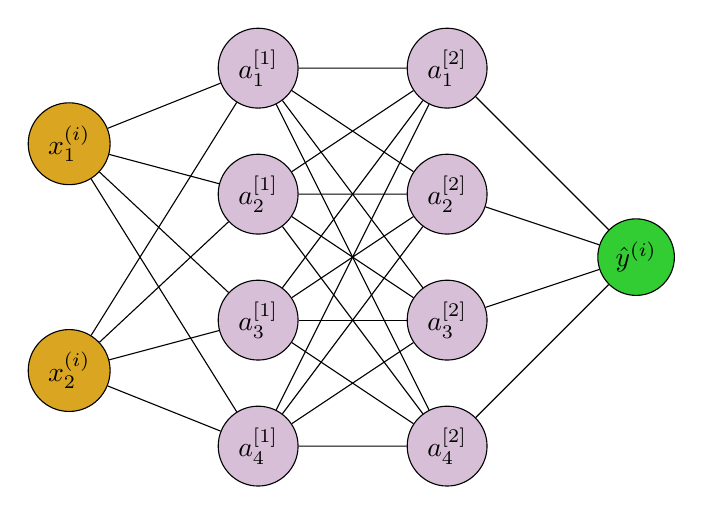
\begin{tikzpicture}[
    every node/.style={circle, draw},
    input/.style={fill=Goldenrod},
    hidden/.style={fill=Thistle},
    output/.style={fill=LimeGreen},
    scale=0.8
]

    % Input Layer
    \node[input] (i1) at (0, 2.8) {$x_1^{(i)}$};
    \node[input] (i2) at (0, -0.8) {$x_2^{(i)}$};

    % Hidden Layer 1
    \node[hidden] (h1) at (3, 4) {$a_1^{[1]}$};
    \node[hidden] (h2) at (3, 2) {$a_2^{[1]}$};
    \node[hidden] (h3) at (3, 0) {$a_3^{[1]}$};
    \node[hidden] (h4) at (3, -2) {$a_4^{[1]}$};

    % Hidden Layer 2
    \node[hidden] (h5) at (6, 4) {$a_1^{[2]}$};
    \node[hidden] (h6) at (6, 2) {$a_2^{[2]}$};
    \node[hidden] (h7) at (6, 0) {$a_3^{[2]}$};
    \node[hidden] (h8) at (6, -2) {$a_4^{[2]}$};

    % Output Layer
    \node[output] (o1) at (9, 1) {$\hat{y}^{(i)}$};

    % Connections 
    \foreach \i in {1, 2} {
        \foreach \j in {1, 2, 3, 4} {
            \draw (i\i) -- (h\j);
        }
    }
    \foreach \i in {1, 2, 3, 4} {
        \foreach \j in {5, 6, 7, 8} {
            \draw (h\i) -- (h\j);
        }
    }
    \foreach \i in {5, 6, 7, 8} {
        \draw (h\i) -- (o1);
    }
\end{tikzpicture}
\caption{A visualization of a neural network with layers of 2, 8,
         8, and 1}
\end{figure}

As you can see in the diagram above, the input of the $i^\text{th}$
training example is represented with the notation $x_n^{(i)}$ for
integer $n$ as $1$ through the total number of inputs. Similarly,
we usually count the first hidden layer as the first layer, and the
activations are represented as $a_n^{[l]}$ were $l$ represents the
layer and $n$ again as the integer from $1$ through the total number
of neurons in the layer. Finally, we use $\hat{y}^{(i)}$ to
represent the prediction for the $i^\text{th}$ training example.

Following the convention, we could write a single neuron as the
following. Note that you might be familiar with $\sigma$ instead
of $g$, but here let's use $g$ for activation function as
$\sigma$ usually represents sigmoid.

\begin{theorem}
{Formula for a Neuron}
{Formula for a Neuron}
For $z_i^{[l]}$ defined as the following, the activation of a neuron
can be represented as the following.
\begin{align*}
    z_i^{[l]}
    &= \sum_{j} w_{ij}^{[l]} a_j^{[l - 1]} + b_i^{[l]} \\
    a_i^{[l]}
    &= g \left( z_i^{[l]} \right)
     = g \left(
            \sum_{j} w_{ij}^{[l]} a_j^{[l - 1]} + b_i^{[l]}
    \right)
\end{align*}
\end{theorem}

One reason why linear algebra is so important in machine learning
is because we could represent the entire layer with simple
matrix operations. Consider the following example for the second
layer.
\[
\begin{bmatrix}
    w_{11}^{[2]} & w_{12}^{[2]} & w_{13}^{[2]} & w_{14}^{[2]}
    \\[0.7em]
    w_{21}^{[2]} & w_{22}^{[2]} & w_{23}^{[2]} & w_{24}^{[2]}
    \\[0.7em]
    w_{31}^{[2]} & w_{32}^{[2]} & w_{33}^{[2]} & w_{34}^{[2]}
    \\[0.7em]
    w_{41}^{[2]} & w_{42}^{[2]} & w_{43}^{[2]} & w_{44}^{[2]}
\end{bmatrix}
\begin{bmatrix}
    a_1^{[1]} \\[0.7em]
    a_2^{[1]} \\[0.7em]
    a_3^{[1]} \\[0.7em]
    a_4^{[1]}
\end{bmatrix}
+
\begin{bmatrix}
    b_1^{[2]} \\[0.7em]
    b_2^{[2]} \\[0.7em]
    b_3^{[2]} \\[0.7em]
    b_4^{[2]}
\end{bmatrix}
=
\begin{bmatrix}
    a_1^{[2]} \\[0.7em]
    a_2^{[2]} \\[0.7em]
    a_3^{[2]} \\[0.7em]
    a_4^{[2]}
\end{bmatrix}
\]
Similarly, we could write different notations for updates.

\begin{theorem}
{Adjusting Parameters with Gradient Descent}
{Adjusting Parameters with Gradient Descent}
Let $l_i$, $b_i$, $J$, and $\eta$ represent weight, bias,
cost function, and learning rate respectively. The new weight and
bias can be represented with the following formula.
\begin{align*}
    w_2 &= w_1 - \eta \frac{\partial J}{\partial w_1} \\
    b_2 &= b_1 - \eta \frac{\partial J}{\partial b_1}
\end{align*}
\end{theorem}

As you can see above, we normally use the cost function $J$ than
the loss function $L$ as the cost function captures the entire loss
while the loss function only represent the loss per example.
Now that we discussed the basic notations and mathematical formulas
for the concepts that we discussed, let's take a look at math in
backpropagation.

\subsection{Deriving Equations and Backpropagation}

Personally it took me a while to fully understand backprop to the
state where I would be able to build a vanilla neural net from
scratch. Here, I would like to share more in-depth understanding
of backpropagation across numerous layers.

To be honest, it took me few days to understand it since I decided
to study mainly because I didn't understand the delta rule. After
reading this note, I highly recommend please try and write your
own network without assistance from LLMs. I though I understood
backprop, which in reality was only the last layer. That
understanding is probably all you need to build the first thing
that we will create in the next section. However, I was stuck
when trying to do backprop across numerous layers. To discuss
this, I thought it would be helpful for us to actually rebuild
or derive main equations involved in a neural network and backprop,
so let's start with that. If you haven't already, please read
the first note if you are unfamiliar with derivatives of multivariable
functions as I won't be going over them here.

Before we derive generalized equations, let's start with a simple
neural net that has two hidden layers, 2 inputs, 3 neurons in each
hidden layer, and two outputs. That way, we can track the indices
for matrices.

\begin{figure}[H]
\centering
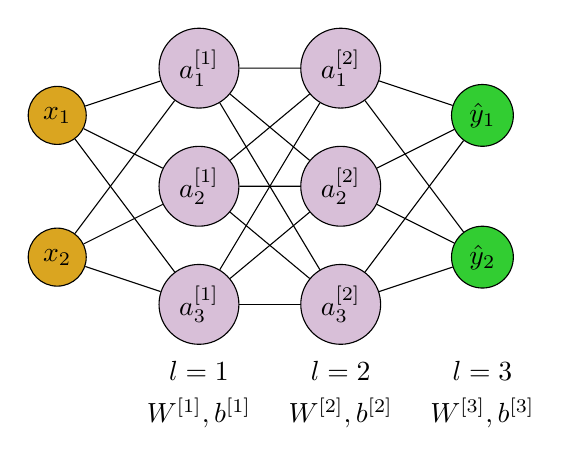
\begin{tikzpicture}[
    input/.style={circle, draw, fill=Goldenrod},
    hidden/.style={circle, draw, fill=Thistle},
    output/.style={circle, draw, fill=LimeGreen},
    scale=0.6
]

    % Input Layer
    \node[input] (i1) at (0, 4) {$x_1$};
    \node[input] (i2) at (0, 1) {$x_2$};

    % Hidden Layer 1
    \node[hidden] (h1) at (3, 5) {$a_1^{[1]}$};
    \node[hidden] (h2) at (3, 2.5) {$a_2^{[1]}$};
    \node[hidden] (h3) at (3, 0) {$a_3^{[1]}$};

    % Hidden Layer 2
    \node[hidden] (h4) at (6, 5) {$a_1^{[2]}$};
    \node[hidden] (h5) at (6, 2.5) {$a_2^{[2]}$};
    \node[hidden] (h6) at (6, 0) {$a_3^{[2]}$};

    % Output Layer
    \node[output] (o1) at (9, 4) {$\hat{y}_1$};
    \node[output] (o2) at (9, 1) {$\hat{y}_2$};

    % Connections 
    \foreach \i in {1, 2} {
        \foreach \j in {1, 2, 3} {
            \draw (i\i) -- (h\j);
        }
    }
    \foreach \i in {1, 2, 3} {
        \foreach \j in {4, 5, 6} {
            \draw (h\i) -- (h\j);
        }
    }
    \foreach \i in {4, 5, 6} {
        \foreach \j in {1, 2} {
            \draw (h\i) -- (o\j);
        }
    }

    \node at (3, -1.4) {$l = 1$};
    \node at (3, -2.3) {$W^{[1]}, b^{[1]}$};
    \node at (6, -1.4) {$l = 2$};
    \node at (6, -2.3) {$W^{[2]}, b^{[2]}$};
    \node at (9, -1.4) {$l = 3$};
    \node at (9, -2.3) {$W^{[3]}, b^{[3]}$};
\end{tikzpicture}
\caption{A visualization of a neural network with layers of 2, 3,
         3, and 2}
\end{figure}

For simplicity, let's use MSE for our loss function, but we will
be generalizing it later. Since $L_1 = \frac{1}{2}
(\hat{y}_1 - y_1)^2$ and $L_2 = \frac{1}{2} (\hat{y}_2 - y_2)^2$,
the following equation is obtained.
\[
L
= \sum_{k = 1}^2 \frac{1}{2} (\hat{y}_k - y_k)^2
\]
Moreover, the preactivation output of the second hidden layer can
be written as following.
\[
\begin{bmatrix}
    z_1^{[2]} \\[0.7em]
    z_2^{[2]} \\[0.7em]
    z_3^{[2]}
\end{bmatrix}
=
\begin{bmatrix}
    w_{11}^{[2]} & w_{12}^{[2]} & w_{13}^{[2]} \\[0.7em]
    w_{21}^{[2]} & w_{22}^{[2]} & w_{23}^{[2]} \\[0.7em]
    w_{31}^{[2]} & w_{32}^{[2]} & w_{33}^{[2]}
\end{bmatrix}
\begin{bmatrix}
    a_1^{[1]} \\[0.7em]
    a_2^{[1]} \\[0.7em]
    a_3^{[1]}
\end{bmatrix}
+
\begin{bmatrix}
    b_1^{[2]} \\[0.7em]
    b_2^{[2]} \\[0.7em]
    b_3^{[2]}
\end{bmatrix}
\]
From the matrix multiplication above, we can write a single output
as the following.
\begin{align*}
    z_2^{[2]}
    &= w_{21}^{[2]} a_1^{[1]} + w_{22}^{[2]} a_2^{[1]} +
        w_{23}^{[2]} a_3^{[1]} + b_2^{[2]} \\
    &= \sum_{j = 1}^3 w_{2j}^{[2]} a_j^{[1]} + b_2^{[2]}
\end{align*}
Now keep in mind the indices! The $2$ in $w_{2j}$ and $b_2$ is the
same $2$ as $z_2$. Generalizing for our cases, we can write the
preactivation outputs as the following.
\[
z_i^{[2]}
= \sum_{j = 1}^3 w_{ij}^{[2]} a_j^{[1]} + b_i^{[2]}
\]
Nice, now that we have the forward pass for our examples, let's
generalize all equations that we have now. For MSE, we could
write it as the following.
\[
L
= \sum_k \frac{1}{2} (\hat{y}_k - y_k)^2
\]
For individual preactivation output, we could write it as the
following equation where $n$ represents the number of neurons
in layer $l-1$.
\[
z_i^{[l]}
= \sum_{j = 1}^n w_{ij}^{[l]} a_j^{[l-1]} + b_i^{[l]}
\]
Now with the equations in mind, let's get into a more confusing
but fun part with loss and gradient. This part is important!
We are not computing the loss of individual neurons. We will
be computing \textit{gradients} instead. Loss will typically be
calculated once with the final outputs.

Let's start with the last layer. Remember! This is the last layer.
To make it more special, let's use $l_f$ to denote the final layer.
\[
\frac{\partial L}{\partial w_{ij}^{[l_f]}}
= \frac{\partial L}{\partial a_{i}^{[l_f]}}
    \frac{\partial a_i^{[l_f]}}{\partial z_i^{[l_f]}}
    \frac{\partial z_i^{[l_f]}}{\partial w_{ij}^{[l_f]}}
\]
In this chain rule here, we don't add other gradients because it is
the last layer. The weights for the output layer does not go through
other paths, but straight to the loss. That's why we don't add
gradients. This would be different for different layers. Using the
definition, MSE, and activation function $g$, the following equation
is obtained.
\[
\frac{\partial L}{\partial w_{ij}^{[l_f]}}
= \left( a_i^{[l_f]} - y_i \right) g'\left( z_i^{[l_f]} \right)
    a_j^{[l_f - 1]}
= \delta_i^{[l_f]} a_j^{[l_f - 1]}
\]
Notice that $\delta_i^{[l_f]}$ will be different depending on the
loss function that we use. To address that and to make our lives
easier for hidden layers, we define $\delta_i^{[l]}$ as the following.
\[
\delta_i^{[l]}
= \frac{\partial L}{\partial z_i^{[l]}}
= \frac{\partial L}{\partial a_i^{[l]}}
    \frac{\partial a_i^{[l]}}{\partial z_i^{[l]}}
\]
Again, because the path from $z_i$ to $a_i$ does not require
additional paths, we do not add other gradients. Now here comes the
\textbf{delta rule}. Let's start deriving them together. Consider
the following equation.
\begin{align*}
    \frac{\partial L}{\partial a_i^{[l]}}
    &= \sum_j \left( \frac{\partial L}{\partial z_j^{[l+1]}}
        \frac{\partial z_j^{[l+1]}}{\partial a_i^{[l]}} \right) \\
    &= \sum_j \delta_j^{[l+1]} w_{ji}^{[l]}
    = \sum_j w_{ji}^{[l]} \delta_j^{[l+1]}
\end{align*}
Substituting back to the definition of $\delta_i^{[l]}$, the
following equation is obtained by the \textbf{delta rule}.
\[
\delta_i^{[l]}
= g'\left(z_i^{[l]}\right) \sum_j w_{ji}^{[l]} \delta_j^{[l+1]}
\]
However, writing all that for each gradient is quite tedious.
Therefore, we get our general formula shown below, which will be
used to build our vanilla MLP.
\[
\frac{\partial L}{\partial w_{ij}^{[l]}}
= \delta_i^{[l]} a_j^{[l-1]}
\]
That was for the weights. Good news is that bias is more simple!
Consider the following equation.
\[
\frac{\partial L}{\partial b_i^{[l]}}
= \frac{\partial L}{\partial a_i^{[l]}}
    \frac{\partial a_i^{[l]}}{\partial z_i^{[l]}}
    \frac{\partial z_i^{[l]}}{\partial b_i^{[l]}}
= \delta_i^{[l]} \frac{\partial z_i^{[l]}}{\partial b_i^{[l]}}
= \delta_i^{[l]}
\]
Now with that formulas and learning rate $\eta$, we can update
the weights and biases as shown in Theorem \ref{theo:Adjusting
Parameters with Gradient Descent}. There are more advanced concepts
like Jacobian matrix for ease in representing, but this is pretty
much it with backprop. Calculating the gradients and updating
based on the loss.

\end{document}


